%-----------------------------------------------------------------------
% Functional Programming 4
% John O'Donnell, Wim Vanderbauwhede
%-----------------------------------------------------------------------

\documentclass{beamer}
%include polycode.fmt
%format alpha = "\alpha"
%format ~> = "\leadsto "
\usepackage{jtodlecseriesFP4}
\usepackage{url}
% Identify this presentation
\SetPresentationTitle
  {Introduction}
  {Introduction}
\SetPresentationNumber
  {1}
\SetPresentationDate
  {Week 1-1}
  {Week 1-1}

%-----------------------------------------------------------------------
% Beginning

\begin{document}

\begin{frame}
  \PresentationTitleSlide
\end{frame}

\begin{frame}
 \frametitle{Topics}
 \tableofcontents
\end{frame}


%-----------------------------------------------------------------------
\section{The FP4 course}

\begin{frame}
\frametitle{The subject of Functional Programming 4}

\begin{itemize}
\item Principles, practice, and (a little) theory of pure
  functional programming
\item Study Haskell, the most widely used functional language
%\item Go deeply into the language, its tools, and its libraries
\item Master the fundamental techniques, including recursion,
  combinators, algebraic data types, equational reasoning, and
  monads.
\item Learn how to write substantial practical programs.
\item Introduce some recent developments and powerful techniques in
  programming: data/task parallelism, software transactional
  memory, automatic testing, generic programming, metaprogramming,
  exotic types.
\end{itemize}
\end{frame}
%-----------------------------------------------------------------------
\begin{frame}
\frametitle{Approach}

\begin{itemize}
\item There are many functional languages.
\item We will focus on Haskell, which is arguably the most
  important functional language (both for research and practical
  applications)
\item The course will begin at the beginning (although we assume you know at least one other programming language)
\item The course will move quickly and get into advanced and powerful
  techniques

\end{itemize}

\end{frame}

%-----------------------------------------------------------------------

%-----------------------------------------------------------------------
\begin{frame}[fragile]
\frametitle{The FutureLearn page}

\begin{itemize}
\item The FutureLearn course page will contain lecture slides, exercises,
  software, pointers to further reading, and announcements.
\item Here is the direct URL:
\end{itemize}

%\begin{verbatim}
\url{https://www.futurelearn.com/courses/functional-programming-in-haskell}
%\end{verbatim}

\end{frame}
%-----------------------------------------------------------------------
%\begin{frame}
%\frametitle{Assessment}
%
%\begin{itemize}
%\item FP4 is assessed through coursework (20\%) and exam (80\%).
%\item There will be one mandatory assessed exercise 
%\item and one \emph{optional} assessed exercise.
%\item If you only do the mandatory assessed exercise it is worth 20\%;
%\item if you do both, the mandatory assessed exercise is 15\% and the optional one 5\%.
%\end{itemize}
%
%\end{frame}

%-----------------------------------------------------------------------
\section{Programming paradigms}

\begin{frame}
\frametitle{Programming paradigms}

There are several major programming paradigms:

\begin{itemize}
\item {\bluetext Imperative languages.}  A program is a set of
  commands telling the computer what to do; by obeying the commands
  the computer solves the problem.
  \begin{itemize}
  \item {\bluetext Basic imperative languages} {\redtext (Fortran,
      Algol60, PL/I, Algol68, C, Pascal, $\ldots$)}
  \item {\bluetext Object oriented languages} {\redtext (Simula67,
      C++, Objective C, Java, $\ldots$)}
  \end{itemize}
\item {\bluetext Declarative languages.}  A program is a
  mathematical description of the solution to a problem; by
  simplifying the description the computer solves the problem.
  \begin{itemize}
  \item {\bluetext Impure functional languages} {\redtext (Lisp,
      ML, Caml, MetaOCaml, $\dots$)}
  \item {\bluetext Pure functional languages} {\redtext (Lisp, FP,
      SASL, KRC, Miranda, Haskell, $\dots$)}
  \item {\bluetext Logic languages} {\redtext (Prolog, Mercury,
      $\ldots$)}
  \end{itemize}
\end{itemize}

\end{frame}
%-----------------------------------------------------------------------
\section{Functional Languages}
\begin{frame}
\frametitle{What are Functional Languages?}

\begin{itemize}
%\item The main current activity in logic languages is how to integrate them with functional languages.
\item There are three main families of functional languages
\item Each family has produced a sequence of experimental
  languages; the most important current one is emphasised:
  \begin{itemize}
  \item Untyped impure: Lisp, {\bluetext Scheme, LiveScript}
  \item Typed impure: ML, Standard ML, {\bluetext OCaml}
  \item Typed pure: ISwim, FP, SASL, KRC, Miranda, {\bluetext
      Haskell}
  \end{itemize}

\item Haskell was designed by the (academic) pure FP community, to enable everyone to use the same basic language design.
\item There are many others, e.g. LiveScript was designed by a community of people who need JavaScript but prefer functional programming.
\end{itemize}

\end{frame}
%-----------------------------------------------------------------------
\begin{frame}
\begin{center}
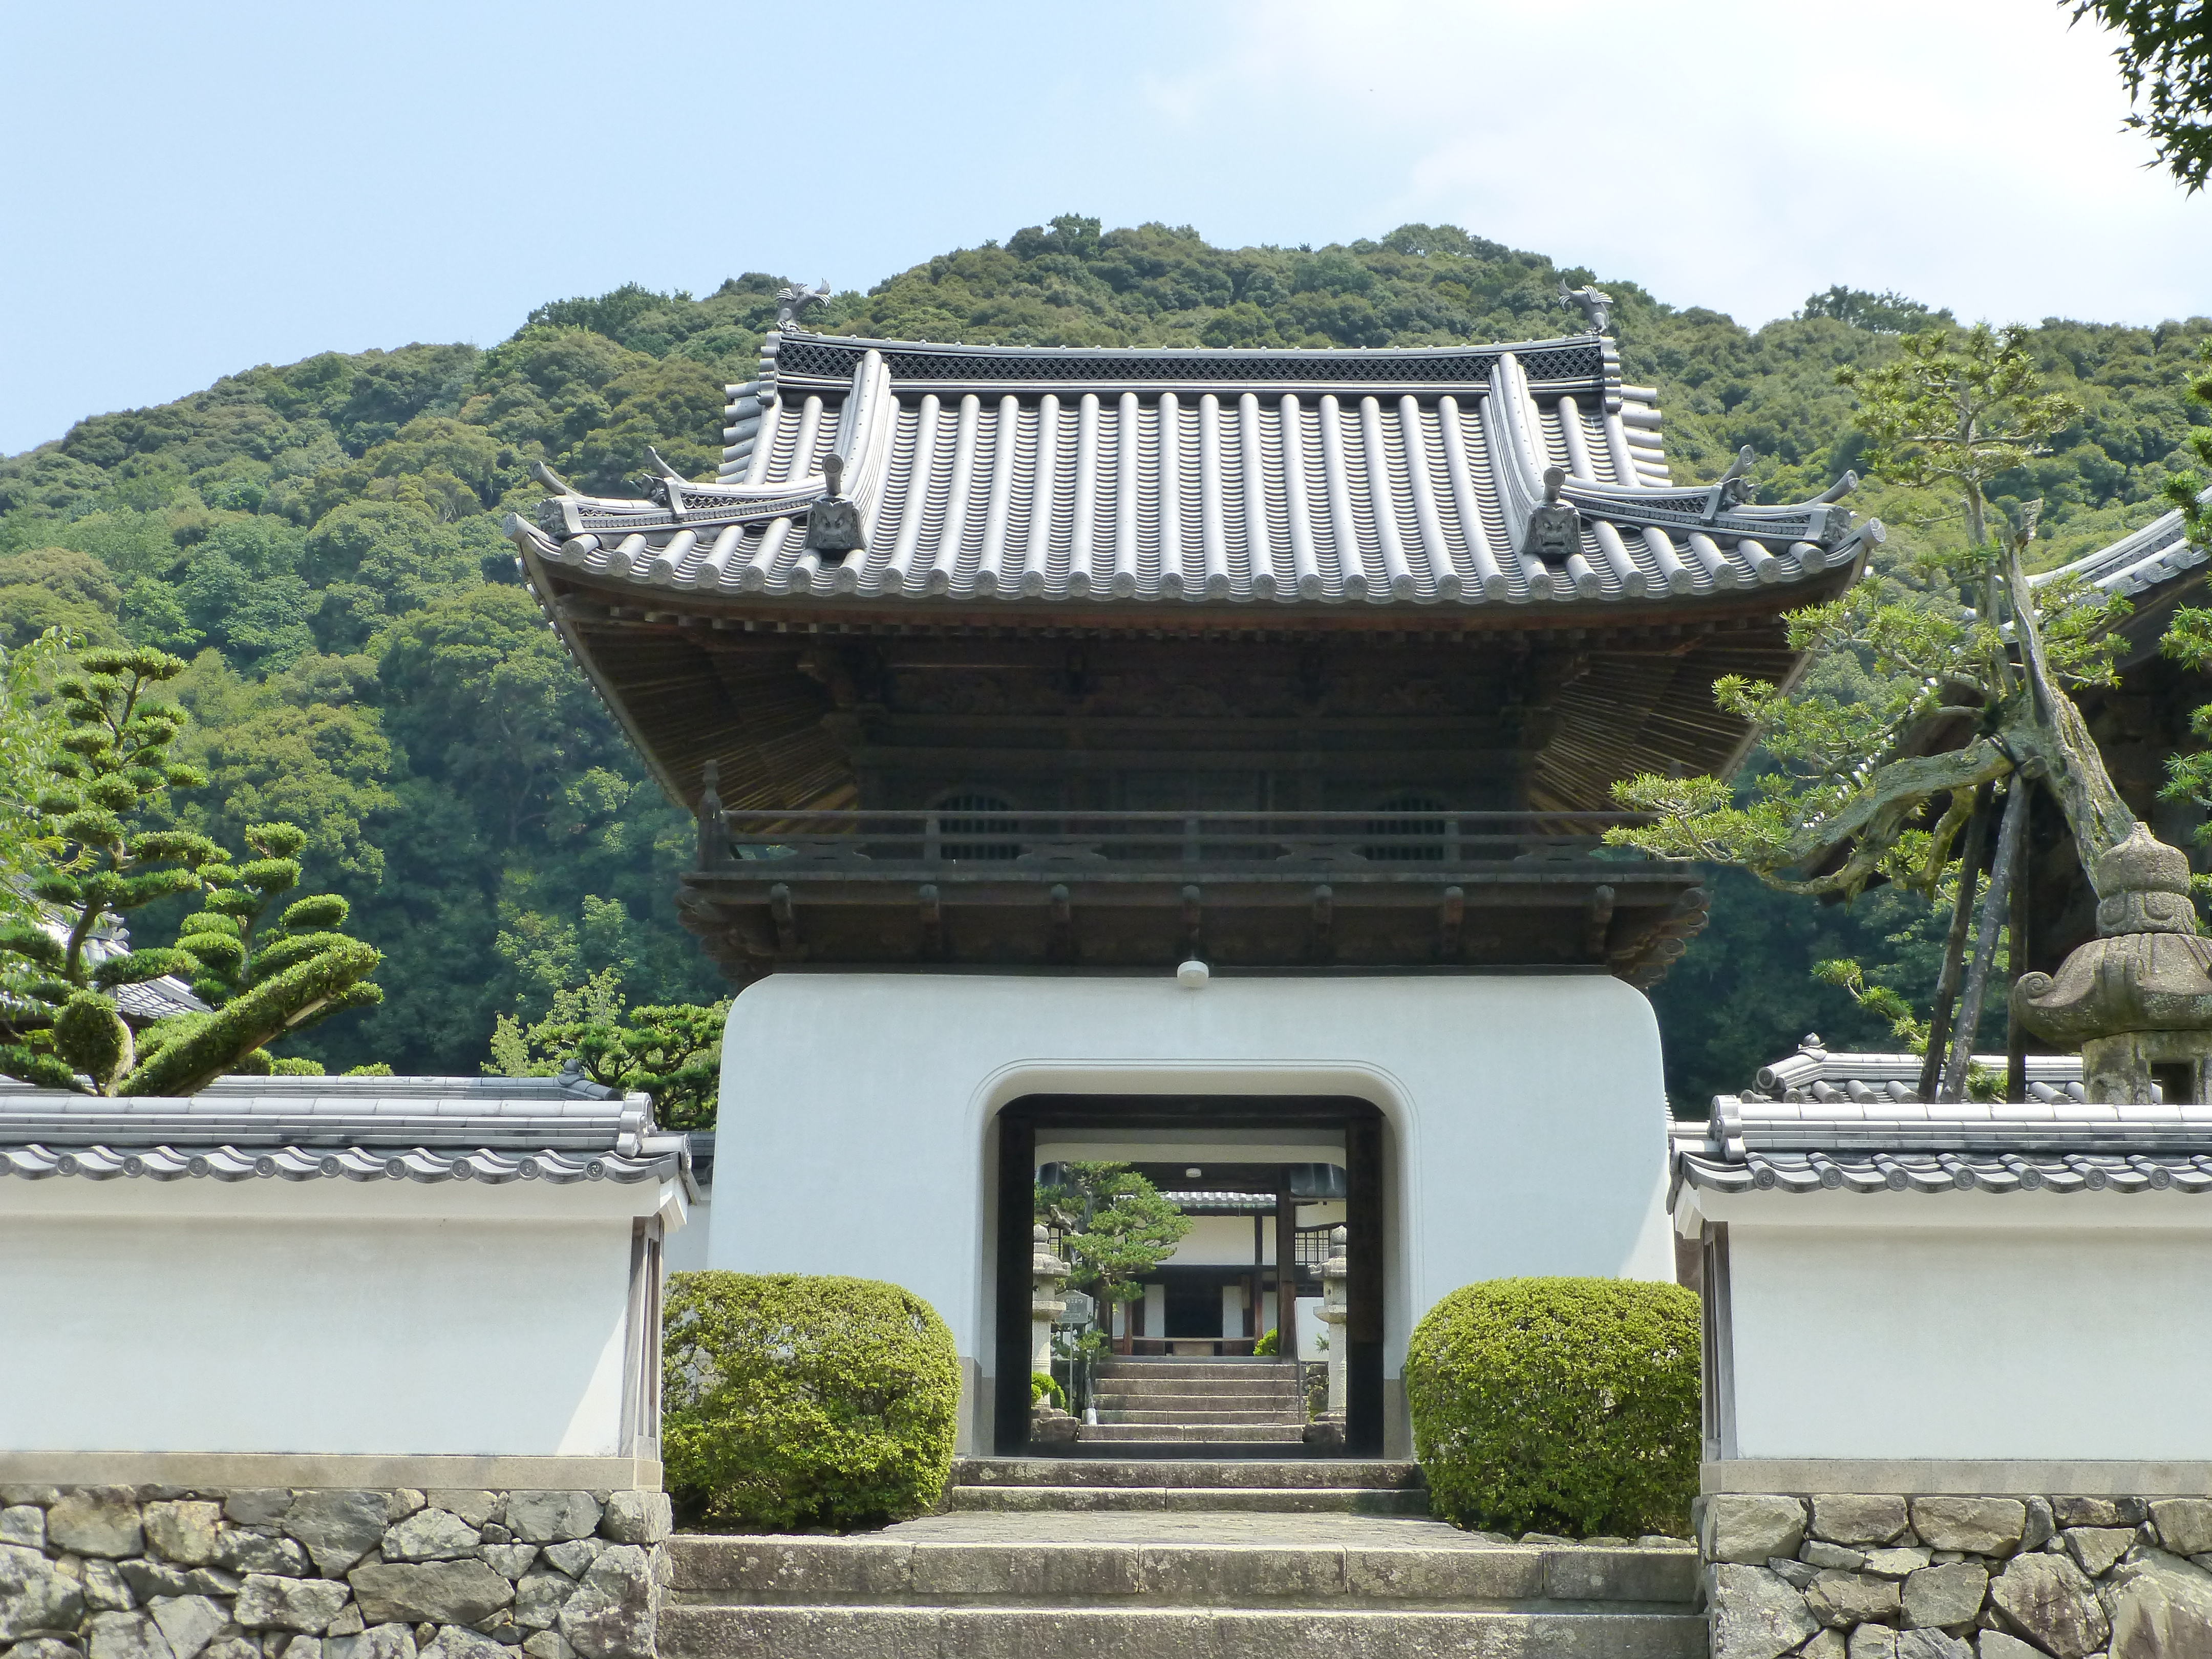
\includegraphics[scale=0.075]
	{figures/jpg/pic01.jpg}
\end{center}
\end{frame}
%-----------------------------------------------------------------------

%\begin{frame}
%\frametitle{What is LiveScript like?}
%
%\begin{itemize}
%\item A small set of general foundational features; everything
%  else is built on top of them.
%\item LiveScript programs tend to be shorter than programs in
%  languages like Java, JavaScript and C++ (sometimes as much as a factor of
%  10).
%\item It's ``dynamically typed'': you generally don't think much about the types of objects.
%\item A central theme in LiveScript is ease of use, obtained through abstraction.
%\end{itemize}
%
%\end{frame}
%-----------------------------------------------------------------------

\begin{frame}
\frametitle{What is Haskell like?}

\begin{itemize}
\item A small set of general foundational features; everything
  else is built on top of them.
\item Haskell programs tend to be shorter than programs in
  languages like Java and C++ (sometimes as much as a factor of
  10).
\item It's ``typeful'': you typically spend half or more than half
  of your time thinking about types.
\item The rich type system requires a lot of thought, but it
  greatly simplifies programming
\item Many errors that would be runtime bugs in other languages are
  caught by the Haskell compiler
\item A central theme in Haskell is abstraction
\item Haskell has a mathematical flavour, and you can use
  mathematics to prove correctness, improve efficiency, and derive
  programs.
\end{itemize}

\end{frame}

%-----------------------------------------------------------------------
\begin{frame}
\frametitle{Pure functional programming}

\begin{itemize}
\item Haskell is \emph{functional}.
  \begin{itemize}
  \item Functions are ``first class'' --- they are ordinary values.
  \item Higher order functions allow the definition of combinators,
    which are something like user-defined language constructs.
  \end{itemize}
\item Haskell is \emph{pure}
  \begin{itemize}
  \item There are no \emph{side effects}.
  \item You don't compute by modifying variables; you compute by
    calculating new values.
  \item Programs are expressions defined with equations and
    functions; programs are executed by \emph{reducing the
      expressions}.
  \item Equations mean real mathematical equality; they are not
    assignment statements.
  \item Haskell is closely related to mathematics.
  \end{itemize}
\end{itemize}

\end{frame}

%-----------------------------------------------------------------------
%-----------------------------------------------------------------------
\begin{frame}
  \frametitle{Functional languages are used in industry}

\begin{itemize}
\item Commercial Users of Functional Programming (CUFP) workshop
  has been meeting annually since 2004 --- {\bluetext @www.cufp.org@}
  \item {\bluetext Intel} uses functional programming for {\redtext
      digital circuit design}
  \item {\bluetext Facebook} uses Haskell for some projects
  \item Galois uses Haskell for {\redtext cryptography}
  \item Several major {\bluetext banks} use Haskell for {\redtext
      financial modeling of derivatives}
  \item Metaweb uses fp for {\redtext web database}
  \item {\bluetext Ericson} uses Erlang for {\redtext telephone
      switching systems}
  \item {\bluetext Microsoft} is incorporating functional
    programming into {\redtext F\#} and {\redtext Visual Studio},
    and some fp concepts are in {\redtext C\#}
  \item SSH uses fp for {\redtext communication security software}
  \item Liveops uses OCaml for a {\redtext Network Services
      Platform}
  \item LiveScript is used in production by SocialText and import.io.      
  \item And many more $\ldots$
\end{itemize}

\end{frame}

%-----------------------------------------------------------------------
\begin{frame}
\frametitle{Haskell is used in research}

\begin{itemize}
\item Functional programming is central to modern research in
  programming languages
\item Haskell has far more research activity than other functional
  languages
\item Most programming language research is about a specific topic,
  not just designing a new language
\item Usually these new topics are explored in functional
  languages, most often in Haskell
\item Some {\bluetext current hot topics:}
  \begin{itemize}
  \item Dependent type systems
  \item Software transactional memory
  \item Task and data parallelism
  \item Hot plugins
  \item Automatic test generation
  \item Correctness proofs of safety-critical software
  \item Metaprogramming
  \item Domain specific languages
  \end{itemize}
\end{itemize}

\end{frame}

%-----------------------------------------------------------------------
\begin{frame}
\frametitle{Programming language concepts}

Many concepts that were developed in functional programming have
been adopted by imperative languages.  (Dates are approximate)

\begin{itemize}
\item Automatic storage management and garbage collection (now in
  Java)
  \begin{itemize}
  \item Lisp, 1960
  \end{itemize}
\item Higher order functions (now in Python)
  \begin{itemize}
  \item Lisp (1960), ISwim (1965), Scheme (1975)
  \end{itemize}
\item Polymorphism (now in Java, C++)
  \begin{itemize}
  \item ML
  \end{itemize}
\item Algebraic data types
  \begin{itemize}
  \item Miranda (1985)
  \end{itemize}
\item Metaprogramming (now in C++)
  \begin{itemize}
  \item Lisp, Planner, Conniver, Scheme, MetaOCaml, Haskell
  \end{itemize}
\item Concurrency with software transactional memory
  \begin{itemize}
  \item Haskell (2005)
  \end{itemize}
\end{itemize}

\end{frame}

%-----------------------------------------------------------------------
\begin{frame}
\frametitle{A bit of history}

\begin{itemize}
\item Functional programming has deep ties to mathematics and
  philosophy.
\item Some if its central concepts were discovered by
  mathematicians in the early and mid 20th century.
\item There is a very deep mathematical theory underlying
  functional programming, consisting of several branches of
  mathematics (predicate logic, lambda calculus, combinatory logic,
  domain theory, denotational semantics, and category theory).
  \begin{itemize}
  \item Don't worry---you don't have to know any of these!
  \end{itemize}
\item The main focus of FP4 is on practical programming and
  advanced techniques
\item But we'll take a little look at some of these other issues,
  to appreciate the richness of the culture of functional
  programming.
\end{itemize}

\end{frame}

%-----------------------------------------------------------------------
\begin{frame}
\frametitle{Famous people}

A very incomplete list of some of the founders of the subject: 

\begin{itemize}
\item Moses Sch\"onfinkel (1889--1942), discovered combinatory
  logic and the technique known as ``currying''.  You'll use
  currying every day, and the Haskell compiler uses a modified form
  of combinatory logic as it translates your program to machine
  language.
\item Alonzo Church (1903--1995), invented the lambda calculus,
  which is the foundation of all functional languages.
\item John Rosser (1907--1989) collaborated with Church, and
  together they proved the \emph{Church-Rosser theorem}, which is
  central to reliability of functional languages, and is the
  fundamental reason that Haskell is considered a leading candidate
  for parallel programming on multicore chips.
\item Haskell Curry (1900--1982) developed combinatory logic
  further, giving it the flexibility that was later exploited by
  functional languages.  \emph{The language Haskell was named after
    him, with the approval of his widow.}
\end{itemize}

\end{frame}

%-----------------------------------------------------------------------
\section{Expressions}

\begin{frame}
\frametitle{Expressions in Haskell}

\begin{itemize}
\item In an imperative language like C or Java,
  \begin{itemize}
  \item there are expressions that denote small scale computations
    (2*x), and
  \item  \emph{statements} that handle sequencing, looping,
    conditionals, and all the large scale operation of the program.
  \end{itemize}
\item \emph{Pure functional programming languages don't have any statements} --- no
  assignments, no jumps.
\item Instead, \emph{all computation is performed by evaluating
    expressions}
\item So, let's start with expressions!
  \begin{itemize}
  \item (We'll still be working on expressions at the end of the
    course, since that's all there is.)
  \end{itemize}
\end{itemize}

\end{frame}
%-----------------------------------------------------------------------

\begin{frame}[fragile]
\frametitle{Examples of integer expressions}

An expression evaluates to a result (usually written $e \rightsquigarrow r$ but we'll use \texttt{e -- > r}).  Haskell uses a similar notation for numbers and operators as most languages:

\begin{verbatim}
2 -- > 2
\end{verbatim}

\begin{verbatim}
3+4 -- > 7
\end{verbatim}

\begin{verbatim}
3+4*5    {equivalent to 3+(4*5)} -- > 23
\end{verbatim}

\begin{verbatim}
(3+4)*5   {equivalent to 7*5} -- > 35    
\end{verbatim}

\end{frame}

%-----------------------------------------------------------------------
\begin{frame}
\frametitle{Syntax of expressions}

\begin{itemize}
\item Parentheses are used for grouping, just as in mathematics. 
\item If you don't need parentheses for grouping, they are
  optional.
\item Operators have precedence, e.g. $*$ has ``tighter''
  precedence than $+$, so $2+3*4$ means $2+(3*4)$.
\item Use reference documentation for complete list of operators
  and their precedences, if you need them.
%\item Warning!  Don't write just -3 to get the number "negative
 % three", you often need to write (-3).
\end{itemize}
\end{frame}

%%%% OK TO HERE %%%
\begin{frame}[fragile]
\frametitle{Function applications}

\begin{itemize}
\item A function takes argument(s), performs some computation, and
  produces result(s).
\item The function $abs$ gives the absolute value of a number.
\item To use a function, you apply it to an argument.  Write the
  function followed by the argument, separated by a space.
\end{itemize}

\begin{verbatim}
abs 5 -- > 5
\end{verbatim}

\begin{verbatim}
abs (-6) -- > 6
\end{verbatim}

\end{frame}

%-----------------------------------------------------------------------
\begin{frame}[fragile]

\frametitle{Parentheses are for grouping}

Good style

\begin{verbatim}
2+3*5
2+(3*5)     {might be clearer to some readers}
abs 7
\end{verbatim}

You don't need parentheses.  The following are legal, but they look
silly:

\begin{verbatim}
(2) + ((3+(((((5)))))))
abs (5)
abs (((5)))
\end{verbatim}

\end{frame}

%-----------------------------------------------------------------------

%-----------------------------------------------------------------------
\begin{frame}[fragile]
\frametitle{Functions with several arguments}

\begin{itemize}
\item $min$ and $max$ are functions that take two arguments.
\item The arguments are given after the function,  separated by
  whitespace. 
\item Write $min\; 3\; 8$, don't write $min(3,8);$
\end{itemize}

\begin{verbatim}
  min 3 8
-- >
  3

  max 3  8
-- >
  8
\end{verbatim}

\end{frame}

%-----------------------------------------------------------------------
\begin{frame}
\frametitle{Precedence of function application}

\begin{itemize}
\item Function application binds tighter than anything else.
\item So \texttt{f x + 3} means \texttt{(f x) + 3} and not \texttt{f (x+3)}
\item If an argument to a function is an expression, you'll need to
  put it in parentheses.
\end{itemize}

\end{frame}

%-----------------------------------------------------------------------
\section{Equations}

\begin{frame}[fragile]
\frametitle{Equations}

\begin{itemize}
\item Equations are used to give names to values.
\end{itemize}

\begin{verbatim}
answer = 42
\end{verbatim}
\end{frame}

%-----------------------------------------------------------------------
\begin{frame}
\frametitle{Equations give names to values}

\begin{itemize}
\item An equation in Haskell is a mathematical equation: it says
  that the left hand side and the right hand side denote the same
  value.
\item The left hand side should be a name that you're giving a
  value to.
  \begin{itemize}
  \item Correct: \texttt{x = 5*y}
  \item Incorrect: \texttt{2 * x = (3*x)**2} -- Reassignment is not allowed in a pure FPL
  \end{itemize}
\end{itemize}

\end{frame}

%-----------------------------------------------------------------------
\begin{frame}[fragile]
\frametitle{Equations are not assignments}

\begin{itemize}
\item A name \emph{can be given only one value}.
\item Names are often called ``variables'', but they \emph{do not
    vary}.
\item In Haskell \emph{variables are constant}!
 
\end{itemize}

\begin{verbatim}
n = 1    -- just fine!
x = 3*n  -- fine
n = x    -- Wrong: can have only one definition of n
\end{verbatim}

\begin{itemize}
\item Once you give a value to a name, you can never change it!
\item This is part of the meaning of ``pure'' and
  ``no side effects''
\end{itemize}

\end{frame}

%-----------------------------------------------------------------------

\begin{frame}
\frametitle{What about n = n+1?}

\begin{itemize}
\item In imperative languages, we frequently say $n := n+1$.
  \begin{itemize}
  \item This is an assignment, not an equation!
  \item It means (1) compute the right hand side, using the old
    value of $n$; then (2) discard the old value of $n$ and
    overwrite it with the new value.
  \item \emph{There are no equations in imperative languages like C
      and Java.}
  \end{itemize}
\item In Haskell, it is valid to write $n = n+1$.
  \begin{itemize}
  \item This is an equation, not an assignment!
  \item It means: compute the value of $n$ that has the property
    that $n = n+1$.
  \item Haskell will try, and it will fail.
\end{itemize}
\end{itemize}

\end{frame}




%-----------------------------------------------------------------------
\begin{frame}
\frametitle{How can you compute without assignments?}

\begin{itemize}
\item Think of an assignment statement as doing three things:
  \begin{enumerate}
  \item It evaluates the right hand side: computing a useful value.
  \item It discards the value of the variable on the left hand
    side: destroying a value that might or might not be useful.
  \item It saves the useful value of the RHS into the variable.
  \end{enumerate}
\item In a pure functional language
  \begin{itemize}
  \item We never destroy old values.
  \item We just compute new useful ones.
  \item If the old value was truly useless, the garbage collector
    will reclaim its storage.
  \end{itemize}
\end{itemize}

\end{frame}

%-----------------------------------------------------------------------
\section{The Haskell interpreter ghci}



%-----------------------------------------------------------------------
\begin{frame}[fragile]
\frametitle{Launching ghci}

To launch the  Haskell interpreter \emph{ghci}:
{\footnotesize
\begin{verbatim}
[wim@fp4 ~]$ghci
GHCi, version 7.8.3: http://www.haskell.org/ghc/  :? for help
Loading package ghc-prim ... linking ... done.
Loading package integer-gmp ... linking ... done.
Loading package base ... linking ... done.
Prelude> 
\end{verbatim}
}

Evaluate an expression

\begin{verbatim}
ls> 3+4
7
\end{verbatim}

\end{frame}

%-----------------------------------------------------------------------
\begin{frame}
\frametitle{Try Haskell!}

\begin{itemize}
\item You can install the Haskell compiler/interpreter on your own computer. Go to \url{https://www.haskell.org/platform} to get the Haskell Platform for your system, it is very easy to install.

\item \emph{All software used in this course is free software.}
\item Try experimenting with the expressions shown in this lecture.
\item And try some experiments of your own.
\end{itemize}

\end{frame}






\end{document}
